\documentclass[fleqn,a4paper,12pt]{article}
\usepackage{standalone}		% Zum Einlesen aus anderen .tex-Files
\usepackage{geometry}		% Zur Bearbeitung des Layouts (Ränder,...)
\geometry{left=30mm, right=40mm, bottom=30mm}
\usepackage[german]{babel}
\usepackage[utf8]{inputenc}
\usepackage{amsmath}		% Mathematische Symbole
\usepackage{amssymb}     	% Nochmehr mathematische Symbole
\usepackage{dsfont}      	% Schriftsatz fuer Zahlenmengensymbole
%\usepackage{verbatim}   	% erweiterte Verbatim-Umgebung
\usepackage{alltt}       	% Quasi-Verbatim-Umgebung
\usepackage{fancyhdr}    	% Eigene Kopfzeilen
\usepackage{graphicx}    	% Zum Einbinden von Grafiken
% Einbinden einer eps-Grafik geht so: includegraphics{path}
\usepackage{wrapfig}
\usepackage{lscape}
\usepackage{rotating}
\usepackage{epstopdf}

% Skalierung der Grafiken
\setlength{\unitlength}{1cm}

\pagestyle{fancy}            % Eigene Kopfzeilen verwenden
\frenchspacing               % Kein Extrafreiraum nach Satzzeichen
\setlength{\parindent}{0pt}  % Neue Absaetze nicht einruecken
%\sloppy                     % Schlampige Absatzformatierung
\fussy                       % Penible Absatzformatierung
\linespread{1.5}             % Zeilenabstand

%andere Definitionen
\newcommand{\R}{{\mathbb R}}
\newcommand{\N}{{\mathbb N}}
\newcommand{\Z}{{\mathbb Z}}
\newcommand{\Q}{{\mathbb Q}}
\newcommand{\C}{{\mathbb C}}
\newcommand{\F}{\mathcal{F}}
\newcommand{\less}{\setminus}
\newcommand{\inv}{{}^{-1}}
\newcommand{\Land}{\bigwedge}
\newcommand{\Lor}{\bigvee}

\begin{document}
Übungsaufgabe 4: \newline
Messreihe Summe der Augenzahlen bei 1000 Würfe mit zwei Würfeln: \newline
9, 9, 9, 7, 7, 6, 5, 8, 7, 8, 10, 8, 7, 2, 4, 11, 6, 7, 7, 4, 6, 8, 7, 6, 12, 6, 4, 5, 7, 3, 5, 8, 6, 8, 7, 6, 6, 9, 3, 8, 7, 6, 6, 10, 11, 12, 4, 7, 7, 8, 9, 4, 5, 10, 3, 11, 8, 8, 7, 9, 8, 7, 11, 2, 8, 5, 8, 6, 9, 11, 8, 9, 11, 8, 6, 8, 5, 8, 5, 11, 4, 7, 7, 3, 3, 10, 10, 7, 8, 5, 8, 6, 8, 3, 12, 5, 7, 4, 5, 9, 8, 6, 7, 11, 7, 7, 3, 9, 12, 5, 9, 6, 5, 8, 3, 10, 7, 11, 7, 4, 11, 3, 9, 4, 7,10, 2, 11, 4, 5, 10, 7, 3, 7, 7, 10, 11, 7, 4, 7, 3, 9, 6, 7, 8, 6, 7, 6, 8, 7, 10, 6, 4, 8, 9, 6, 7, 11, 11, 9, 8, 6, 6, 11, 9, 9, 4, 8, 5, 4, 4, 4, 7, 7, 8, 10, 5, 7, 9, 9, 7, 5, 8, 5, 8, 8, 3, 7, 5, 7, 4, 7, 8, 8, 5, 6, 4, 5, 10, 9, 4, 5, 3, 6, 5, 7, 7, 11, 5, 7, 8, 8, 5, 5, 6, 7, 6, 6, 7, 5, 9, 11, 8, 6, 6, 11, 8, 5, 8, 6, 3, 5, 3, 3, 10, 11, 8, 5, 12, 9, 11, 7, 10, 9, 7, 6, 11, 9, 7, 3, 8, 7, 2, 6, 6, 7, 4, 10, 5, 8, 7, 6, 4, 6, 9, 4, 9, 6, 10, 4, 5, 10, 11, 8, 4, 6, 10, 5, 3, 7, 8, 2, 8, 9, 6, 5, 11, 6, 5, 11, 7, 8, 6, 12, 6, 6, 10, 4, 6, 9, 10, 6, 4, 7, 7, 8, 10, 10, 4, 3, 9, 9, 9, 3, 12, 4, 12, 8, 9, 12, 10, 11, 3, 8, 8, 5, 6, 8, 10, 7, 3, 11, 5, 7, 8, 5, 5, 6, 6, 7, 7, 10, 6, 8, 4, 4, 8, 12, 5, 7, 5, 6, 4, 7, 3, 9, 3, 11, 7, 8, 4, 7, 7, 4, 5, 9, 8, 8, 2, 6, 5, 4, 6, 5, 5,8, 9, 8, 11, 5, 9, 5, 8, 6, 8, 7, 3, 8, 7, 6, 6, 7, 4, 8, 7, 8, 10, 5, 5, 7, 8, 6, 4, 6, 8, 6, 6, 9, 7, 9, 5, 11, 10, 5, 7, 9, 8, 6, 12, 6, 10, 9, 3, 4, 5, 7, 7, 7, 4, 5, 7, 3, 9, 6, 6, 8, 11, 7, 8, 7, 7, 4, 2, 9, 5, 4, 6, 5, 4, 6, 4, 5, 5, 8, 11, 4, 9, 4, 5, 9, 8, 7, 6, 12, 8, 6, 9, 3, 8, 7, 6, 5, 7, 8, 5, 6, 7, 9, 5, 5, 11, 6, 5, 8, 8, 4, 4, 9, 6, 7, 8, 12, 8, 8, 8, 5, 7, 7, 7, 12, 5, 6, 10, 12, 9, 2, 5, 8, 6, 4, 4, 4, 6, 9, 8, 2, 4, 6, 8, 8, 2, 9, 9, 8, 7, 3, 5, 9, 6, 7, 10, 9, 9, 6, 3, 8, 8, 6, 6, 10, 6, 6, 7, 5, 7, 8, 10, 7, 7, 11, 9, 10, 8, 10, 9, 9, 6, 3, 4, 6, 5, 7, 10, 3, 6, 7,8, 3, 10, 7, 11, 7, 9, 10, 8, 9, 5, 6, 9, 8, 8, 6, 5, 9, 6, 2, 4, 11, 5, 11, 10, 7, 6, 6, 10, 4, 6, 6, 3, 5, 12, 4, 4, 11, 2, 8, 9, 7, 8, 9, 8, 7, 6, 3, 8, 9, 8, 9, 8, 7, 4, 10, 6, 4, 5, 6, 5, 7, 5, 6, 8, 10, 5, 3, 8, 11, 4, 6, 7, 7, 2, 8, 8, 10, 7, 4, 11, 6, 4, 5, 4, 10, 5, 8, 7, 7, 4, 6, 7, 6, 7, 8, 6, 6, 3, 9, 4, 3, 7, 10, 12, 10, 5, 6, 8, 9, 9, 7, 4, 5, 9, 8, 3, 9, 7, 3, 6, 6, 6, 6, 8, 7,2, 12, 6, 5, 7, 8, 8, 10, 7, 5, 6, 8, 5, 3, 10, 7, 6, 8, 11, 9, 10, 8, 7, 3, 6, 8, 4, 6, 6, 3, 4, 11, 3, 10, 6, 3, 3, 12, 9, 7, 5, 7, 3, 6, 8, 5, 3, 5, 7, 9, 2, 5, 10, 8, 8, 10, 9, 12, 5, 8, 7, 7, 9, 5, 9, 10, 12, 7, 8, 4, 10, 12, 3, 7, 9, 4, 5, 12, 10, 7, 9, 12, 9, 5, 10, 2, 9, 6, 9, 4, 5, 5, 9, 7, 5, 4, 9, 7, 5, 11, 6, 4, 11, 6, 7, 7, 8, 6, 7, 4, 6, 11, 4, 5, 8, 4, 5, 7, 4, 4, 7, 7, 2, 2, 7, 11, 9, 6, 5, 6, 6, 6, 9, 7, 4, 8, 6, 4, 10, 7, 6, 6, 4, 3, 6, 5, 9, 8, 2, 9, 8, 2, 5, 6, 7, 9, 4, 3, 3, 5, 3, 4, 2, 7, 4, 2, 9, 6, 5, 5, 7, 4, 5, 10, 2, 8, 5, 5, 8, 6, 4, 8, 4, 7, 6, 7, 7, 5, 4, 2, 10, 8, 7, 4, 7, 8, 8, 9, 7, 8, 3, 4, 10, 2, 8, 12, 6, 11, 10, 7, 9, 7, 4, 6, 12, 3, 6, 7, 7, 3, 9, 6, 6, 6, 10, 6, 5, 6, 4, 3, 6, 5, 7, 5, 4, 4, 6, 8, 9, 10, 10, 7, 10, 5, 6, 12, 5, 5, 7, 9, 9, 7,11, 6, 8, 6, 7, 7, 6, 6, 12, 10, 12, 7, 6, 4, 4, 3, 8, 6, 11, 4, 2, 4, 7, 10, 10, 5, 7, 5, 9, 11, 8, 3, 12, 5, 8, 6, 7, 6, 7, 8, 9, 11, 5, 4, 6, 8, 5, 6, 6, 6, 10, 7, 12, 7, 9, 7 \newline
\textbf{Häufigkeiten}
\begin{center}
	\begin{tabular}{ | l | l | l | }
		\hline
		Summe der Augenzahlen & Anzahl der Würfe & relative Häufigkeit \\ \hline
		2 & 26 & 0.026 \\ \hline
		3 & 59 & 0.059 \\ \hline
		4 & 97 & 0.097 \\ \hline
		5 & 118 & 0.118 \\ \hline
		6 & 153 & 0.153 \\ \hline
		7 & 162 & 0.162 \\ \hline
		8 & 138 & 0.138 \\ \hline
		9 & 98 & 0.098 \\ \hline
		10 & 68 & 0.068 \\ \hline
		11 & 50 & 0.05 \\ \hline
		12 & 31 & 0.031 \\ \hline
	\end{tabular}  
\end{center}
\textbf{Median:} 7 \newline
\textbf{Modalwert:} 7 \newline
\textbf{Mittwelwert:} 6.847 \newline
\textbf{Standardabweichung:} $\approx 2.4$ \newline
\textbf{Entropie:} $\approx 3.2658$ \newline
\textbf{Max. Entropie:} $\approx 3.4594$ \newline
\textbf{Redundanz:} $\approx 0.194$ \newline
\begin{figure}
	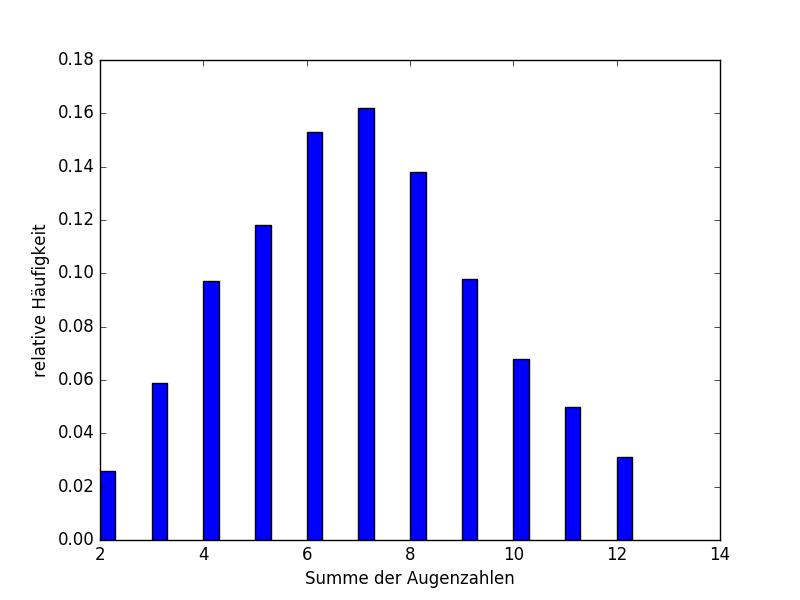
\includegraphics[width=1.0\textwidth]{A04_histo1.png}
	\caption{Normales Histogramm für die Summe der Augenzahlen mit zwei Würfeln bei 1000 Würfen}
\end{figure}
\begin{figure}
	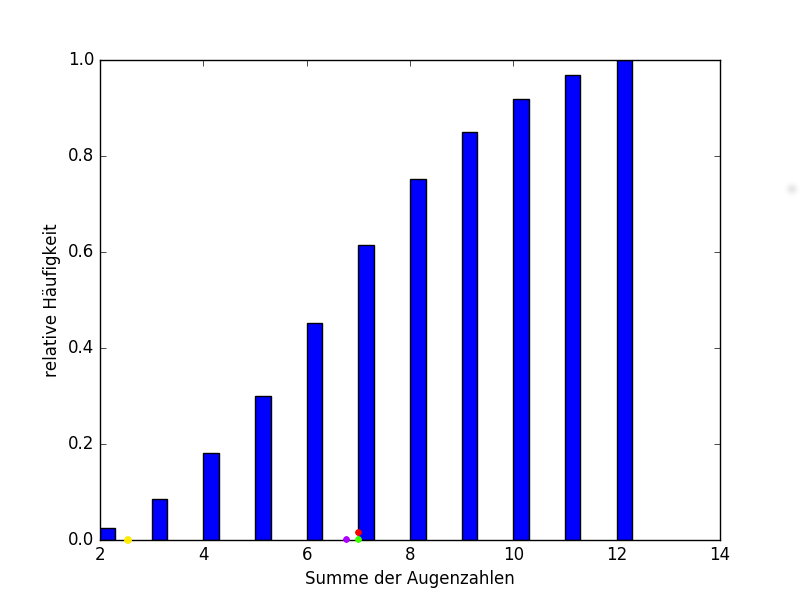
\includegraphics[width=1.0\textwidth]{A04_histo2.png}
	\caption{Kumulative Histogramm für die Summe der Augenzahlen mit zwei Würfeln bei 1000 Würfen \newline gelb: Standardabweichung, rot: Modalwert, grün: Median, violett: Mittwelwert}
\end{figure}
\end{document}